% MiKTeX 的 etex.sty v2.7 不再定义 \reserveinserts，WileyNJDv5.cls 仍会调用它。
\providecommand{\reserveinserts}[1]{}
\documentclass[APA,STIX1COL,doublespace]{WileyNJDv5}
\usepackage{setspace}
\geometry{a4paper,margin=25mm,headheight=21pt,headsep=11pt,footskip=36pt}

\articletype{Original Article}
\historydates{}
\doiheadtext{}
\startpage{1}
\makeatletter
\abs@coli@hsize=.28\textwidth
\abs@colii@hsize=.68\textwidth
\long\def\absworkarea#1#2{\par\noindent
  \begin{minipage}[t]{\abs@coli@hsize}#1\end{minipage}\hfill
  \begin{minipage}[t]{\abs@colii@hsize}#2\end{minipage}\par}
\def\oddfoot@titlepage@info{\hbox to \textwidth{\hfill\pagenumfont\thepage}}
\let\evenfoot@titlepage@info\oddfoot@titlepage@info
\def\oddhead@titlepage@info{}
\let\evenhead@titlepage@info\oddhead@titlepage@info
\makeatother

\hypersetup{hidelinks,pdftitle={Joint Profile Inference for High Dimensional Mixed Effects Quantile Regression with Many Small Clusters},pdfauthor={Jian Hou, Tan Meng, and Maozai Tian}}

\DeclareMathOperator*{\argmin}{arg\,min}
\DeclareMathOperator{\Var}{Var}
\DeclareMathOperator{\Cov}{Cov}
\DeclareMathOperator{\diag}{diag}
\newcommand{\E}{\mathbb{E}}
\newcommand{\R}{\mathbb{R}}
\newcommand{\Heff}{H_{\mathrm{eff}}}
\newcommand{\Oeff}{\Omega_{\mathrm{eff}}}
\newcommand{\supp}{Supporting Information}
\newcommand{\MilkCows}{1349}
\newcommand{\MilkSamples}{2253}
\newcommand{\MilkRepeatCows}{904}
\newcommand{\MilkRepeatSamples}{1808}
\newcommand{\MilkOriginalCows}{1356}
\newcommand{\MilkOriginalSamples}{2270}
\newcommand{\MilkInvalidCows}{7}
\newcommand{\MilkInvalidSamples}{17}
\newcommand{\MilkSpectra}{1060}
\newcommand{\MilkDimension}{1073}
\newcommand{\MilkAOneCows}{519}
\newcommand{\MilkATwoCows}{830}
\newcommand{\MilkFits}{18}
\newcommand{\MilkSystems}{72}
\newcommand{\MilkMinSelected}{27}
\newcommand{\MilkMaxSelected}{163}
\newcommand{\MilkMedianRuntime}{17.0}
\newcommand{\MilkMaxKKT}{5.17e-09}
\newcommand{\MilkMaxNuisance}{9.99e-11}
\newcommand{\MilkSpectralCorrelation}{0.9986}
\newcommand{\MilkLowerEstimate}{-0.020}
\newcommand{\MilkLowerSE}{0.101}
\newcommand{\MilkLowerInterval}{[-0.263,\ 0.223]}
\newcommand{\MilkMedianEstimate}{0.018}
\newcommand{\MilkMedianSE}{0.118}
\newcommand{\MilkMedianInterval}{[-0.264,\ 0.299]}
\newcommand{\MilkUpperEstimate}{0.119}
\newcommand{\MilkUpperSE}{0.140}
\newcommand{\MilkUpperInterval}{[-0.216,\ 0.453]}

\newcommand{\JointActiveCoverage}{0.964}
\newcommand{\JointActiveMCSE}{0.004}
\newcommand{\JointActiveAblationCoverage}{0.935}
\newcommand{\JointActiveCoverageDifference}{0.028}
\newcommand{\JointActiveDifferenceMCSE}{0.004}
\newcommand{\JointActiveLength}{0.275}
\newcommand{\JointActiveAblationLength}{0.259}
\newcommand{\JointNullCoverage}{0.968}
\newcommand{\JointNullMCSE}{0.003}
\newcommand{\JointNullAblationCoverage}{0.956}
\newcommand{\JointNullCoverageDifference}{0.012}
\newcommand{\JointNullDifferenceMCSE}{0.004}
\newcommand{\JointNullLength}{0.315}
\newcommand{\JointNullAblationLength}{0.286}
\newcommand{\JointDatasets}{1440}
\newcommand{\JointIntervals}{5760}
\newcommand{\JointAblationShiftCount}{306}
\newcommand{\JointAblationMaxShift}{0.350}
\newcommand{\JointWeakCoverage}{0.958}
\newcommand{\JointWeakAblationCoverage}{0.803}
\newcommand{\JointWeakDifference}{0.156}
\newcommand{\JointWeakDifferenceMCSE}{0.022}
\newcommand{\JointRuntimeFiveHundred}{0.966}
\newcommand{\JointRuntimeTenThousand}{9.976}
\newcommand{\JointSingleMinimumOrder}{1.003}
\newcommand{\JointSingleMaximumOrder}{1.014}
\newcommand{\JointPairMinimumOrder}{1.998}
\newcommand{\JointPairMaximumOrder}{2.000}
\newcommand{\JointModuleWorkflows}{52}
\newcommand{\JointModulePairedFits}{6760}
\newcommand{\JointPlasmaALowerEstimate}{-0.133}
\newcommand{\JointPlasmaALowerScoreInterval}{[-0.213, -0.054]}
\newcommand{\JointPlasmaALowerWorkflowInterval}{[-0.222, -0.045]}
\newcommand{\JointPlasmaAMedianEstimate}{-0.091}
\newcommand{\JointPlasmaAMedianScoreInterval}{[-0.163, -0.019]}
\newcommand{\JointPlasmaAMedianWorkflowInterval}{[-0.168, -0.013]}
\newcommand{\JointPlasmaAUpperEstimate}{-0.057}
\newcommand{\JointPlasmaAUpperScoreInterval}{[-0.123, 0.009]}
\newcommand{\JointPlasmaAUpperWorkflowInterval}{[-0.125, 0.011]}
\newcommand{\JointPlasmaBLowerEstimate}{-0.068}
\newcommand{\JointPlasmaBLowerScoreInterval}{[-0.144, 0.009]}
\newcommand{\JointPlasmaBLowerWorkflowInterval}{[-0.151, 0.015]}
\newcommand{\JointPlasmaBMedianEstimate}{-0.065}
\newcommand{\JointPlasmaBMedianScoreInterval}{[-0.122, -0.008]}
\newcommand{\JointPlasmaBMedianWorkflowInterval}{[-0.126, -0.003]}
\newcommand{\JointPlasmaBUpperEstimate}{-0.036}
\newcommand{\JointPlasmaBUpperScoreInterval}{[-0.089, 0.018]}
\newcommand{\JointPlasmaBUpperWorkflowInterval}{[-0.092, 0.021]}
\newcommand{\JointGeneRoles}{360}
\newcommand{\JointGeneIntervals}{1080}
\newcommand{\JointLowerGeneA}{PTTG1}
\newcommand{\JointLowerGeneCountA}{11}
\newcommand{\JointLowerGeneB}{PTTG1}
\newcommand{\JointLowerGeneCountB}{6}

\newcommand{\RegisteredJointSettings}{71}
\newcommand{\RegisteredJointDatasets}{45500}
\newcommand{\RegisteredJointFailures}{6}
\newcommand{\RegisteredJointAvailable}{45494}
\newcommand{\RegisteredFullPredictorSettings}{66}
\newcommand{\RegisteredFullActiveCoverage}{0.971}
\newcommand{\RegisteredFullActiveMCSE}{0.001}
\newcommand{\RegisteredFullNullCoverage}{0.977}
\newcommand{\RegisteredFullNullMCSE}{0.001}
\newcommand{\VarianceFilterActiveCoverage}{0.661}
\newcommand{\VarianceFilterNullCoverage}{0.694}
\newcommand{\FullDesignActiveCoverage}{0.977}
\newcommand{\FullDesignNullCoverage}{0.989}
\newcommand{\VarianceFilterSecondShifted}{463}
\newcommand{\VarianceFilterEleventhShifted}{472}


\begin{document}

\title{Joint Profile Inference for High Dimensional Mixed Effects Quantile Regression with Many Small Clusters}

\author[1]{Jian Hou}
\author[1]{Tan Meng}
\author[1]{Maozai Tian}

\authormark{Hou et al.}
\titlemark{Joint profile quantile inference}

\address[1]{\orgdiv{School of Statistics}, \orgname{Renmin University of China}, \orgaddress{\city{Beijing}, \country{China}}}

\corres{Jian Hou, School of Statistics, Renmin University of China, Beijing, China. Email: houjian@ruc.edu.cn}

\abstract[Abstract]{Quantile inference with many small clusters becomes computationally demanding when the fixed-effect dimension is large. We construct a joint profile estimator for the minimiser of the complete ridge-profiled check loss. Outcome and covariate searches select a model for each requested coordinate, which is estimated on independent subjects. The selected target displacement is controlled by a quadratic outcome error and a product of outcome and contrast errors. Pairing convex coefficient fits at two bandwidths removes the first-order smoothing term introduced by nuisance profiling. We establish learning rates, a cluster influence representation and consistent variance estimation. A study of \RegisteredJointDatasets{} datasets examines full target coverage across \RegisteredJointSettings{} settings. Four-coordinate inference with 200 clusters and 10000 predictors takes a median of \JointRuntimeTenThousand{} seconds. An application with \MilkCows{} cows and \MilkSpectra{} spectral predictors finds no statistically resolved A2 milk-type association with somatic cell score after full spectrum adjustment.}

\keywords{clustered data; conditional adjustment; convolution smoothing; high-dimensional inference; mixed-effects model; profile M-estimation; quantile regression}

\maketitle

\section{Introduction}\label{sec:introduction}

Longitudinal quantile regression can involve thousands of predictors and
only a few measurements on each subject. Repeated milk spectra provide
one setting: each sample contains many correlated absorbance measurements,
while persistent animal variation links samples from the same cow
\cite{chirife2025data}. Mixed-effects models represent that
heterogeneity through a small number of subject-specific effects
\cite{pinheiro2000,jiang2007}. When the number of subjects increases but
their visit counts remain bounded, each subject effect continues to be
estimated from limited information. Its treatment affects both the
coefficient being estimated and the uncertainty attached to it.

Quantile regression describes associations across the response
distribution \cite{koenker1978,koenker2005}. Sparse estimation in high
dimension is supported by penalised quantile methods
\cite{belloni2011,wang2012,tan2022}; convolution smoothing also permits
efficient optimisation and distributional inference
\cite{fernandes2021,he2021,yan2023}. Mixed-effects quantile models have
been developed through asymmetric-Laplace working likelihoods and
penalised formulations \cite{geraci2014,geraci2014jss,li2020}.
The many-small-cluster regime brings an incidental-parameter problem
even in low dimension \cite{battagliola2022}. A high-dimensional method
therefore needs a population target that remains meaningful when the
subject effects are estimated from bounded samples.

We use the population minimiser of a complete ridge-profiled check loss.
The criterion averages within subjects and then across independent
subjects. Its nuisance penalty is fixed as part of the parameter
definition. Differentiating the smoothed criterion gives a score in the
original fixed-effect design and a positive Schur-complement curvature
that retains the nuisance ridge. The structural interpretation of a
coordinate follows from a population orthogonality condition. The
profile target also remains defined when the working subject model
approximates the observed heterogeneity.

Dimension reduction presents a further statistical question. A variable
that contributes little to prediction can still be needed to adjust a
coefficient of interest. Post double selection addresses this issue in
high-dimensional regression \cite{belloni2014}, and orthogonal scores
with sample splitting permit inference after nuisance learning
\cite{ning2017,chernozhukov2018}. Orthogonal greedy search offers a
computationally economical learner \cite{ing2011}; its combination with
debiased inference has also been studied \cite{cha2022}. For a complete
quantile profile, the relevant adjustment depends on the population
profile curvature. We learn a profile adjustment set and supplement it
with conditional covariate associations. Their union controls the
change of the target caused by fitting a smaller model. For independent
Gaussian covariate rows, inclusion of the target's conditional
neighbours gives exact preservation of that coordinate even when other
outcome coefficients are omitted.

The estimation sample is independent of its variable-selection sample.
On each selected model we fit the complete profile at two bandwidths.
This pairing addresses a feature of profiling with bounded cluster
sizes: a symmetric smoothing kernel can induce a term linear in the
bandwidth because the nuisance optimiser moves with that bandwidth.
We derive the term through the active faces of the dual score box under
joint-density conditions. Combining the two fitted coefficient vectors
with weights $2$ and $-1$ removes the first-order term. Each fit retains
a positive curvature matrix, and its contribution to the final cluster
variance is computed at its own fitted coefficient.

The computational procedure follows this statistical construction.
High-dimensional search uses a weighted orthogonal basis and certified
joint convex optimisation. Cluster nuisance problems have finite
solution constructions for an intercept and for an intercept with a
time slope. The final coefficient systems have the dimension of the
selected model. We derive approximation rates for the actual search
and validation rules, then bound the selected-model target error by a
quadratic outcome error and a product of outcome and contrast errors.
The resulting paired estimator has a cluster influence representation
and a consistent variance estimate. The argument accommodates
imperfect outcome selection without a minimum nonzero outcome
coefficient condition.

Longitudinal estimating equations and quadratic inference functions
provide related methods for variable selection
\cite{zu2023,song2024,bhattacharya2026}. Testing procedures are also
available for high-dimensional longitudinal mean and quantile models
\cite{fang2020,wang2023}; Gaussian mixed-model inference has been
developed through quasi-likelihood \cite{li2022}. Our construction
addresses the complete quantile profile target and the first-order
smoothing effect created by its nuisance optimisation. Numerical
calculations examine the target approximation and the behaviour of the
implemented intervals. The application uses repeated milk spectra and
somatic cell counts \cite{chirife2025data}. It estimates a prespecified
milk-type coordinate while the complete spectral design supplies the
high-dimensional adjustment variables.

\section{The complete quantile profile and its target}\label{sec:model}

\subsection{Clustered observations}\label{subsec:model}

Let $D_i=\{(Y_{ij},X_{ij},Z_{ij}):j=1,\ldots,m_i\}$ denote cluster
$i$, for $i=1,\ldots,n$. The response is scalar,
$X_{ij}\in\mathbb R^p$ is the fixed-effect design, and
$Z_{ij}\in\mathbb R^q$ describes an intercept or a small collection of
cluster effects. Clusters are independent. Their sizes satisfy
$1\leq m_i\leq m_{\max}<\infty$ in the asymptotic regime, while
$p=p_n$ can exceed $n$ and $q$ remains fixed. A structural model
motivating the criterion is
\begin{equation}\label{eq:structural-model}
 Q_\tau(Y_{ij}\mid X_i,Z_i,b_i)
       =X_{ij}^T\beta^0+Z_{ij}^Tb_i,\qquad \tau\in(0,1).
\end{equation}
The working nuisance design can also approximate cluster
heterogeneity. Every empirical average uses the number of independent
clusters. Averaging the loss within a cluster gives each subject unit
weight, including when visit counts vary.

The fixed-effect design may contain a prespecified set $\mathcal U$
of always-included covariates. The remaining coordinates are eligible
for selection. Target coordinates are specified before their
estimation outcomes are used.

\subsection{An unsmoothed population parameter}\label{subsec:target}

Fix a positive-definite working matrix $\Lambda\in\mathbb R^{q\times q}$.
With $\rho_\tau(u)=u\{\tau-I(u<0)\}$, define
\begin{equation}\label{eq:cluster-unsmoothed}
 \ell_i(\beta,\gamma)=\frac1{m_i}\sum_j
       \rho_\tau(Y_{ij}-X_{ij}^T\beta-Z_{ij}^T\gamma)
                    +\tfrac12\gamma^T\Lambda\gamma.
\end{equation}
The nuisance minimiser
\begin{equation}\label{eq:gamma-target}
 \gamma_i^\dagger(\beta)=\argmin_{\gamma\in\mathbb R^q}
                              \ell_i(\beta,\gamma)
\end{equation}
is unique. The population risk and target are
\begin{equation}\label{eq:population-profile-risk}
 R_0(\beta)=\E\ell_i\{\beta,\gamma_i^\dagger(\beta)\},
 \qquad \beta^\star\in\argmin_{\beta\in\mathbb R^p}R_0(\beta).
\end{equation}
The expectation follows the actual distribution of independent
clusters, including their visit counts. This regularised profile
parameter depends on $\Lambda$ and is defined before introducing a
smoothing bandwidth.

At the nuisance optimum, a dual vector
$s_i\in[\tau-1,\tau]^{m_i}$ satisfies
\[
 \Lambda\gamma_i^\dagger=m_i^{-1}Z_i^Ts_i,\qquad
 s_{ij}\in\partial\rho_\tau
       (Y_{ij}-X_{ij}^T\beta-Z_{ij}^T\gamma_i^\dagger).
\]
It gives the cluster subgradient $-m_i^{-1}X_i^Ts_i$. A joint
conditional outcome density makes the dual vector unique almost surely
at a fixed $\beta$. Its coordinates at zero residuals are determined
by the nuisance stationarity equation. The Supporting Information
establishes this uniqueness and the corresponding smoothing limit.

Under population differentiability and identification, the structural
slope equals the profile target when
\begin{equation}\label{eq:structural-orthogonality}
 \E\{-m_i^{-1}X_i^Ts_i(\beta^0)\}=0.
\end{equation}
Centred fixed-effect covariates independent of the cluster nuisance
design and location-shift errors give this equality for the relevant
slopes. In general, inference concerns the projection in
\eqref{eq:population-profile-risk}. Its definition continues to apply
when the structural interpretation changes.

\subsection{Population targets after dimension reduction}\label{subsec:selected-target}

For a set $A$ containing a target coordinate $k$, let
\begin{equation}\label{eq:selected-population-target}
 \beta_A^P\in\argmin_{\beta:\,\beta_{A^c}=0}R_0(\beta).
\end{equation}
The vector is embedded in $\mathbb R^p$. Its $k$th coordinate can
differ from $\beta_k^\star$ even when the reduced model predicts well.
For example, suppose two centred Gaussian covariates have unit
variances and correlation $\rho$, and are independent of the cluster
errors and nuisance effects. Fitting only the first covariate gives
the profile coefficient $\beta_1^0+\rho\beta_2^0$. With coefficients
$0.4$ and $-0.4$ and correlation $0.5$, that target is $0.2$.
Retaining an adjustment variable can therefore matter before any
standard error is calculated.

Our selected sets approximate both the coefficient vector and the
population contrast for the target. The first approximation controls
profile risk; the second controls the effect of omitted covariates on
the target coordinate. Section~\ref{sec:theory} bounds
$|\beta_{A,k}^P-\beta_k^\star|$ using their product and gives an exact
conditional-covariate result for Gaussian designs.

\subsection{Smoothed profile geometry}\label{subsec:profile-calculus}

Let $K$ be a symmetric density with compact support and define
\begin{equation}\label{eq:smoothed-loss}
 \rho_{\tau,b}(u)=\int\rho_\tau(u-bv)K(v)\,dv,
 \quad \psi_{\tau,b}=\rho_{\tau,b}',\quad
 \phi_{\tau,b}=K_b,\qquad K_b(u)=K(u/b)/b.
\end{equation}
The computations use the Epanechnikov kernel. For $b>0$ put
\begin{equation}\label{eq:cluster-smoothed}
 \ell_{i,b}(\beta,\gamma)=m_i^{-1}\sum_j
 \rho_{\tau,b}(Y_{ij}-X_{ij}^T\beta-Z_{ij}^T\gamma)
                  +\tfrac12\gamma^T\Lambda\gamma,
\end{equation}
and write
\[
 \widehat\gamma_{i,b}(\beta)=\argmin_\gamma\ell_{i,b}(\beta,\gamma),
 \qquad \ell_{i,b}^{\mathrm{prof}}(\beta)
          =\ell_{i,b}\{\beta,\widehat\gamma_{i,b}(\beta)\}.
\]
At residual $r_i=Y_i-X_i\beta-Z_i\widehat\gamma_{i,b}(\beta)$, define
\begin{equation}\label{eq:WiBiAi}
 W_i=m_i^{-1}\diag\{K_b(r_{ij})\},\quad
 B_i=Z_i^TW_iZ_i+\Lambda,\quad A_i=B_i^{-1}Z_i^TW_iX_i.
\end{equation}

\begin{proposition}[Complete profile calculus]\label{prop:profile-calculus}
The cluster profile gradient and Hessian are
\begin{align}
 g_{i,b}(\beta)&=-m_i^{-1}X_i^T\psi_{\tau,b}(r_i),
                                  \label{eq:profile-score}\\
 H_{i,b}(\beta)&=X_i^TW_iX_i-X_i^TW_iZ_iB_i^{-1}Z_i^TW_iX_i.
                                  \label{eq:heff-schur}
\end{align}
With $\widetilde X_i=X_i-Z_iA_i$, the same Hessian equals
\begin{equation}\label{eq:heff-ridge-identity}
 H_{i,b}=\widetilde X_i^TW_i\widetilde X_i+A_i^T\Lambda A_i.
\end{equation}
It is positive semidefinite and satisfies
\begin{equation}\label{eq:schur-variational}
 v^TH_{i,b}v=\min_a
 \{\|W_i^{1/2}(X_iv-Z_ia)\|_2^2+a^T\Lambda a\}.
\end{equation}
\end{proposition}

The envelope theorem gives the gradient. Differentiating nuisance
stationarity yields $\partial\widehat\gamma_{i,b}/\partial\beta^T=-A_i$,
which gives the Schur complement. Completing the square proves
\eqref{eq:schur-variational}. These identities determine the curvature
used for both adjustment selection and the final coefficient fits.

\section{Joint profile estimation and inference}\label{sec:inference}

\subsection{Independent selection and estimation}\label{subsec:roles}

Let $\mathcal K$ be a fixed set of target coordinates. Partition whole
clusters into two estimation folds $I_1,I_2$, with $n_f=|I_f|$, and use
$T_f=I_f^c$ to select the model for $I_f$. The folds are balanced,
so their limiting proportions are positive. All visits of a subject retain
the same role. The always-included set $\mathcal U$ is fixed before
selection. For each $k\in\mathcal K$, the selected set $A_{fk}$ contains
$\mathcal U$ and $k$. The two role assignments use every cluster once
for estimation.

Selection has an outcome component and an adjustment component. The
outcome component approximates the full profile risk. The adjustment
component retains variables needed to keep the target coefficient close
to its full-model value. Section~\ref{sec:theory} states these two
approximation requirements and derives them for the learners below.

\subsection{Outcome search with a joint convex criterion}\label{subsec:search}

On a training set $T$ of $r$ clusters, let
$\widehat\Sigma_T=r^{-1}\sum_{i\in T}X_i^TX_i/m_i$. For a path set
$S$ containing $\mathcal U$, jointly minimise
\begin{equation}\label{eq:search-fit}
 \frac1r\sum_{i\in T}\ell_i(\beta_S,\gamma_i)
       +\frac{1}{2r}\beta_S^T\widehat\Sigma_{T,SS}\beta_S,
 \qquad \beta_{S^c}=0.
\end{equation}
The small prediction ridge is invariant to a change of basis in the
selected span. Weighted QR coordinates make its proximal map explicit.
The complete quantile criterion has a box-constrained dual, and its
primal-dual gap certifies each selected fit. We use the linesearch of
\citeA{malitsky2018} with these proximal maps.

The next variable maximises the absolute dual correlation with the
part of its weighted column orthogonal to the selected span, divided
by the norm of that residual column. This extends orthogonal greedy
search \cite{ing2011} to the complete nonsmooth profile. Every step
examines the full design. The preceding coefficients and dual vector
initialise the enlarged convex problem.

Three inner cluster folds within $T_f$ construct these paths. On a
training subset of size $r$, set
$M_0(r)=\min\{p,\lfloor r/\log r\rfloor,\lceil(\log r)^3\rceil\}$.
The number of added outcome variables is bounded by
\begin{equation}\label{eq:search-budget}
 M_Y(r)=\min\!\left[p-|\mathcal U|,
 \left\{\min\!\left(\left\lfloor\frac r{\log r}\right\rfloor,
                  \left\lceil(\log r)^3\right\rceil\right)
           -|\mathcal U|\right\}_+\right].
\end{equation}
Use the smallest inner training budget as the common path length.
The selected size minimises the total exact heldout profile loss at
bandwidth zero. The union $S_f^Y$ retains the selected path sets from
all three inner fits. It therefore contains the comparison coefficient
vectors that attain the heldout risk bound.

\subsection{Conditional covariates and profile adjustment}\label{subsec:graphs}

Write $H_{i,b}=X_i^TL_{i,b}X_i$, where
\[
 L_{i,b}=W_{i,b}-W_{i,b}Z_i
          (Z_i^TW_{i,b}Z_i+\Lambda)^{-1}Z_i^TW_{i,b}.
\]
The Schur identity makes $L_{i,b}$ positive semidefinite. On an inner
training sample, evaluate its profile at the corresponding outcome
fit and form the rectangular factor with blocks
$F_{i,b}=L_{i,b}^{1/2}X_i$. Standardise each factor column to have unit
cluster-averaged second moment. For target $k$, the nodewise path solves
\begin{equation}\label{eq:nodewise-fit}
 \min_a\left\{\frac{1}{2r}
       \|F_{b,k}^{\circ}-F_{b,-k}^{\circ}a\|_2^2
                   +\lambda\|a\|_1\right\},\qquad b\in\{h,h/2\}.
\end{equation}
Each path is anchored at its zero-solution penalty. Geometric ratios
decrease by $2^{-1/4}$ from one to at most $r^{-1/2}$.

For each ratio, combine the two graph supports with the inner outcome
set and the target. Refit the two positive quadratic nodewise problems
on that set, with ridge $1/r$ times their common reference diagonal.
The sum of their heldout quadratic losses selects the ratio. A graph
union exceeding $M_0(r)$ on its inner training sample is ineligible. The
zero graph remains a candidate. Combining the selected inner sets
gives $S_{fk}^H$.

Conditional covariate regression provides an additional adjustment set.
Its factor has blocks $X_i/\sqrt{m_i}$ and uses no outcome weights.
Five cluster folds choose its nodewise L1 penalty by prediction loss.
The grid has 24 log-spaced ratios from one to
$\min\{0.05,|T_f|^{-1/2}\}$. Retain at most the smallest inner $M_0(r)$
of selected variables, ordered by the absolute standardised regression
coefficients, and call this set $S_{fk}^X$. The final model is
\begin{equation}\label{eq:selected-set}
 A_{fk}=\mathcal U\cup\{k\}\cup S_f^Y\cup S_{fk}^H\cup S_{fk}^X.
\end{equation}
The conditional covariate set can retain a necessary adjustment when
its outcome coefficient is too small to influence prediction-based
selection. Its addition also retains every comparison vector supplied
by the outcome and profile searches.

\subsection{Paired coefficient estimation}\label{subsec:paired-fit}

On $I_f$, use the same set $A=A_{fk}$ at both bandwidths. With
$\widehat\Sigma_{f,A}=n_f^{-1}\sum_{i\in I_f}X_{i,A}^TX_{i,A}/m_i$,
fit
\begin{equation}\label{eq:joint-selected-fit}
 \widehat\beta_{f,b,A}\in\argmin_{\beta_A}
 \left\{\frac1{n_f}\sum_{i\in I_f}\ell_{i,b}^{\mathrm{prof}}(\beta_A)
             +\frac{1}{2n_f^2}\beta_A^T\widehat\Sigma_{f,A}\beta_A\right\},
 \qquad b\in\{h,h/2\}.
\end{equation}
Coefficients outside $A$ are zero. The numerical ridge supplies
positive systems and contributes a vanishing term on the inferential
scale. Newton updates use the exact profile gradient and Schur
curvature, with backtracking on the complete objective.

Let $\beta_{A,b}^P$ minimise the corresponding population profile risk.
The density expansion gives
\begin{equation}\label{eq:coefficient-bandwidth-expansion}
 \beta_{A,b}^P=\beta_A^P+b\,a_A+O(b^2).
\end{equation}
The same selected model at both bandwidths has the same first-order
coefficient $a_A$. Its cancellation leads to
\begin{equation}\label{eq:joint-estimator}
 \widehat\theta_k=\sum_{f=1}^2\frac{n_f}{n}
       \{2\widehat\beta_{f,h/2,A_{fk},k}
                         -\widehat\beta_{f,h,A_{fk},k}\}.
\end{equation}
We use $h=n^{-3/10}$, with declared multipliers in sensitivity
calculations. Both constituent fits minimise convex criteria.

For a prespecified input design, one estimation sample suffices:
take $I_1=\{1,\ldots,n\}$ and include its complete coordinate set.
This case applies to the clinical and module models. An exploratory
design selected on separate subjects uses the same one-fold
calculation for its selected-model parameter $\beta_A^P$.

\subsection{Cluster uncertainty}\label{subsec:variance}

For $A=A_{fk}$ define
\[
 \widehat H_{f,b,A}=\frac1{n_f}\sum_{i\in I_f}
          H_{i,b,AA}(\widehat\beta_{f,b,A})+n_f^{-2}\widehat\Sigma_{f,A},
 \qquad
 \widehat\omega_{f,b,k}=\widehat H_{f,b,A}^{-1}e_{k,A},
\]
where $e_{k,A}$ selects coordinate $k$ within $A$. Each cluster contributes
\begin{equation}\label{eq:joint-influence}
 V_{ik}=-2\widehat\omega_{f,h/2,k}^T
               g_{i,h/2,A}(\widehat\beta_{f,h/2,A})
          +\widehat\omega_{f,h,k}^T
               g_{i,h,A}(\widehat\beta_{f,h,A}),\qquad i\in I_f.
\end{equation}
The gradient uses $X_{i,A}$ from the original design. Combining both
bandwidth contributions within the cluster retains their covariance.
With $\bar V_{fk}=n_f^{-1}\sum_{i\in I_f}V_{ik}$, set
\begin{equation}\label{eq:variance-estimator}
 \widehat s_k^2=\frac1{n^2}\sum_f\sum_{i\in I_f}
                        (V_{ik}-\bar V_{fk})^2.
\end{equation}
The pointwise interval is
\begin{equation}\label{eq:ci}
 \widehat\theta_k\ \pm\ z_{1-\alpha/2}\widehat s_k.
\end{equation}
Section~\ref{sec:theory} establishes its validity for the full profile
target. A prespecified finite family can use Bonferroni allocation.

\subsection{Computational cost and reproducibility}\label{subsec:implementation}

With $N$ rows and $M$ search steps, the complete-design score and
projection updates cost $O(MNp)$. At selected dimension $d$, a joint
primal-dual iteration costs $O(Nd+Nq+nq^2)$. The profile factors are
rectangular, and each final Newton system has dimension $|A_{fk}|$.
The number of requested coordinates multiplies the corresponding
nodewise and selected-fit calculations. The implementation records
actual iterations and numerical residuals together with the sample
roles and selected sets. An incomplete numerical solution remains a
recorded failed attempt.

The computational revision used OpenAI Codex from the GPT-6 family
in October 2026 for assistance with mathematical development and
implementation, following the authors' research objectives and
revision requests. Numerical results are generated by the supplied R
and C++ programs from the declared simulation designs or the public
milk records. The application retains the cow and sample identifiers
provided with that release.

\begin{algorithm}[t]
\caption{Joint profile coordinate inference}\label{alg:estimation}
\begin{algorithmic}[1]
\State Fix $\Lambda$, $h$, $\mathcal U$, the target coordinates and the cluster folds.
\For{each estimation fold $I_f$}
\State Construct outcome search paths on the complementary subjects and select their size by inner profile risk.
\State Learn the profile and conditional covariate adjustment sets on those complementary subjects.
\For{each target $k$}
\State Construct $A_{fk}$ in \eqref{eq:selected-set} and fit \eqref{eq:joint-selected-fit} on $I_f$ at $h$ and $h/2$.
\State Retain the paired coefficient and the cluster contributions in \eqref{eq:joint-influence}.
\EndFor
\EndFor
\State Combine folds using \eqref{eq:joint-estimator} and compute \eqref{eq:variance-estimator} and \eqref{eq:ci}.
\end{algorithmic}
\end{algorithm}

\section{Target preservation and statistical inference}\label{sec:theory}

The theory connects the selected models to the full profile parameter.
The learning samples provide comparison coefficients and contrasts.
Independent estimation then permits a selected-model expansion at
each bandwidth. Throughout, constants are uniform over the triangular
array, and all rates use the number of clusters.

\subsection{Density and design conditions}\label{subsec:assumptions}

\begin{assumption}[Clusters and population regularity]\label{ass:clusters}
The clusters are iid with bounded sizes. Their nuisance designs are
bounded matrices with a fixed number of columns, and the eigenvalues
of the fixed positive-definite $\Lambda$ lie in a positive compact
interval. The kernel is symmetric, compactly
supported and Lipschitz, is positive in its interior, and has an
absolutely continuous inverse distribution function. Conditional on
$(X,Z,m)$, the outcome density belongs to $C^3(\mathbb R^m)$ and obeys
\begin{equation}\label{eq:density-section}
 \sup_{y_A}\int |\partial^\alpha f(y_A,y_B)|\,dy_B\leq C,
 \qquad B=A^c,\quad |\alpha|\leq3,
\end{equation}
for every coordinate partition, with a uniform constant. The profile
risk is finite, has a unique minimiser $\beta^\star$, and the average
absolute response has bounded expectation.
\end{assumption}

\begin{assumption}[Design contrasts and sparse curvature]\label{ass:design}
Conditional on $(Z,m)$, each design contrast $X_j^Tv$ on the relevant
sparse supports has sub-Gaussian norm at most $C\|v\|_2$.
Sparse design eigenvalues are bounded above
and away from zero. On a fixed coefficient ball containing the
considered sparse population minimisers, the complete profile risk has
restricted Hessian eigenvalues in $[\kappa,C]$ and uniformly bounded
third directional derivatives. These bounds hold on the sparse
supports and enlarged supports used in the learning arguments.
\end{assumption}

Independent Gaussian or standardised $t_3$ errors with bounded positive
scales satisfy the density section conditions after arbitrary
conditional location mixing. The curvature argument applies to bounded
nuisance designs of any fixed dimension. The
Supporting Information gives the population and empirical arguments
for these classes.

\begin{theorem}[Population bandwidth expansion]\label{thm:target}
Under Assumptions~\ref{ass:clusters} and \ref{ass:design}, the complete
profile gradient has the expansion
\begin{equation}\label{eq:score-bandwidth-expansion}
 \E g_{i,b}(\beta)=\nabla R_0(\beta)+bB_1(\beta)+O(b^2).
\end{equation}
The corresponding Hessian expands through order $b^2$. The
directional forms are uniform on the stated sparse neighbourhood.
For a selected population model with positive restricted curvature,
\eqref{eq:coefficient-bandwidth-expansion} holds uniformly and
\begin{equation}\label{eq:paired-population-coefficient}
 2\beta_{A,h/2}^P-\beta_{A,h}^P=\beta_A^P+O(h^2).
\end{equation}
\end{theorem}

The linear term in \eqref{eq:score-bandwidth-expansion} arises because
the fitted cluster effect moves with $b$. The proof integrates the
dual score over its active faces. It permits positive probability at
zero for fitted profile residuals.

\subsection{Approximation of the full target}\label{subsec:target-theory}

Write $H_0=\nabla^2R_0(\beta^\star)$. For a target $k$, suppose a
population contrast $c_{0k}$ exists with
\begin{equation}\label{eq:population-direction}
 c_{0k,k}=1,\qquad H_0c_{0k}=J_{0k}e_k,\qquad
 J_{0k}=c_{0k}^TH_0c_{0k}>0,\qquad \omega_{0k}=c_{0k}/J_{0k}.
\end{equation}
Only the contrasts required by the target coordinates enter the
assumptions. Let $e_n$ and $r_n$ describe the outcome and contrast
approximations supplied by selection.

\begin{theorem}[Selected model target]\label{thm:selected-target}
Suppose $A$ contains a comparison coefficient $b_A$ with
$R_0(b_A)-R_0(\beta^\star)=O_p(e_n^2)$ and a comparison contrast
$v_A$ with $v_{A,k}=1$, support in $A$ and
$\|v_A-c_{0k}\|_2=O_p(r_n)$. Under the local population curvature
conditions, with $J_{0k}$ bounded away from zero,
\begin{equation}\label{eq:selected-target-bound}
 \|\beta_A^P-\beta^\star\|_2=O_p(e_n),\qquad
 |\beta_{A,k}^P-\beta_k^\star|=O_p(e_n^2+r_ne_n).
\end{equation}
\end{theorem}

Restricted stationarity gives $v_A^T\nabla R_0(\beta_A^P)=0$.
Expanding at $\beta^\star$ leaves
$J_{0k}(\beta_{A,k}^P-\beta_k^\star)$, a product involving
$v_A-c_{0k}$ and the coefficient error, and a quadratic remainder.
This explains why both components of selection enter
\eqref{eq:selected-target-bound}.

\begin{proposition}[Conditional covariates preserve a Gaussian slope]\label{prop:gaussian-target}
Conditional on the nuisance design and cluster size, suppose the
covariate rows are independent centred Gaussian with covariance
$\Sigma$, and independent of the complete error and nuisance vectors.
For $Y=X\beta^0+Zb+\varepsilon$, the selected population profile
coefficient is, at every bandwidth,
\begin{equation}\label{eq:gaussian-selected-target}
 \beta_{A,A}^P=\beta_A^0+
                 \Sigma_{AA}^{-1}\Sigma_{A,A^c}\beta_{A^c}^0.
\end{equation}
If $\operatorname{supp}(\Sigma^{-1}e_k)\subseteq A$, then
$\beta_{A,k}^P=\beta_k^0$.
\end{proposition}

Gaussian conditional projection makes the omitted design residual
independent of $X_A$. At the coefficient in
\eqref{eq:gaussian-selected-target}, the complete profile score has
mean zero. The stated inverse-row inclusion makes the $k$th row of
$\Sigma_{AA}^{-1}\Sigma_{A,A^c}$ zero. Outcome coefficients can be
omitted while that target coordinate remains unchanged.

\subsection{Rates for the selected sets}\label{subsec:learning-rates}

Assume $\beta^\star$ has at most $s$ nonzero coordinates and bounded
Euclidean norm. The contrast $c_{0k}$ has at most $s_c$ nonzero
coordinates and bounded L1 norm. Let $M$ be the largest inner value
of $M_0(r)$, with the smallest value of the same order. Put
$D=7M+s+s_c+|\mathcal U|+2$ and $L_n=\log(2np)$.
Sparse eigenvalue bounds hold on sufficiently large multiples of the
comparison supports to give the nodewise compatibility conditions.
The graph budget admits the corresponding fixed multiple of $s_c$.

\begin{theorem}[Outcome and contrast learning]\label{thm:learning}
Under the preceding conditions, let $\epsilon_n$ bound the normalised
primal-dual gaps of the initial fits and define
\begin{align}
 \delta_n&=\sqrt{D L_n/n}+(D L_n)^{3/2}/n,
 &\nu_n&=\delta_n+n^{-1}+\sqrt{\epsilon_n},\nonumber\\
 a_n&=\sqrt{D L_n/(nh)}+D L_n/(nh).
 &&\label{eq:learning-fluctuations}
\end{align}
In the regime $a_n+\nu_n\to0$, the selected sets in
\eqref{eq:selected-set} contain the comparison
vectors required by Theorem~\ref{thm:selected-target}, with
\begin{align}
 e_n&=e^{-cM/(2s)}+\sqrt{s}\nu_n+
                              \sqrt{\log(CM)/n},\label{eq:outcome-rate}\\
 r_n&=(1+\sqrt{s_c})(a_n+e_n+h+n^{-1})
                  +\sqrt{\log(CM\log n)/(nh)}.\label{eq:contrast-rate}
\end{align}
The bounds are uniform over the fixed number of outer folds and
requested coordinates.
\end{theorem}

The proof controls nonsmooth profile dual scores uniformly over sparse
sets. It then derives a geometric decrease of population risk along
the greedy path, up to its sampling error. Heldout profile loss selects
a comparison coefficient at that rate. Positive nodewise quadratic
loss gives the contrast comparison. The union of the inner supports
retains these vectors, and the design regression adds at most $M$
coordinates. Outcome coefficients may approach zero at arbitrary
rates within the stated sparsity and norm bounds.

\subsection{Cluster influence representation}\label{subsec:bahadur}

For $b>0$ let $m_b=\E g_{i,b}(\beta^\star)$ and define the centred
triangular-array contribution
\begin{equation}\label{eq:influence}
 \xi_{ik,h}=-\omega_{0k}^T
       [2\{g_{i,h/2}(\beta^\star)-m_{h/2}\}
                         -\{g_{i,h}(\beta^\star)-m_h\}].
\end{equation}
Assume its variance $\sigma_{k,h}^2$ is bounded above and away from
zero. Bounded dual scores and the design contrast condition give
uniform moments above order two. Let $d_n$ bound the selected
estimation dimension.

\begin{theorem}[Paired coefficient inference]\label{thm:bahadur}
Suppose the preceding conditions hold, and
\begin{equation}\label{eq:remainder-conditions}
 \sqrt n(h^2+e_n^2+r_ne_n)\to0,\qquad
 e_n^2/h+r_n^2\to0,\qquad
 \frac{(d_n\log n)^3}{nh}\to0.
\end{equation}
The numerical score residuals contribute $o_p(n^{-1/2})$. Then
\begin{equation}\label{eq:bahadur}
 \sqrt n(\widehat\theta_k-\beta_k^\star)
       =\frac1{\sqrt n}\sum_{i=1}^n\xi_{ik,h}+o_p(1),
\end{equation}
and
\begin{equation}\label{eq:normality}
 \frac{n\widehat s_k^2}{\sigma_{k,h}^2}\longrightarrow_p1,
 \qquad
 \frac{\widehat\theta_k-\beta_k^\star}{\widehat s_k}
                 \rightsquigarrow N(0,1).
\end{equation}
The interval in \eqref{eq:ci} has limiting coverage $1-\alpha$ for
the full profile coordinate.
\end{theorem}

Conditioning on one fold's selection sample fixes its selected model
while preserving independent estimation observations. The selected
population target is controlled by
\eqref{eq:selected-target-bound}; pairing removes its first-order
bandwidth term. The fitted cluster contributions then approach the
same centred population contributions. This conditioning is used
separately for each fold, without treating the two selected sets as
jointly independent of all observations.

In the high-dimensional regime $p\geq n$, for bounded $s$, $s_c$ and
$|\mathcal U|$, take the implemented
asymptotic budget $M=\lceil(\log n)^3\rceil$ and $h=n^{-3/10}$.
A sufficient dimension regime is
\begin{equation}\label{eq:feasible-regime}
 \log(2np)=o\{n^{7/20}/(\log n)^3\}.
\end{equation}
Here the dominant product is controlled by
$D L_n/\sqrt{nh}\to0$, while $\sqrt n h^2=n^{-1/10}$.
Growing sparsities retain the explicit requirements
\eqref{eq:outcome-rate}--\eqref{eq:remainder-conditions}. For a
prespecified fixed design, the selection approximation terms vanish
and the same paired-fit argument applies with one estimation sample.

\section{Numerical studies}\label{sec:simulation}

\subsection{Population movement under smoothing}\label{subsec:smoothing-example}

The repeated observation model permits a direct calculation of the
coefficient pairing. A cluster contains two identical observations
$Y\sim N(0,1)$, with $X=Z=1$ and $\Lambda=\lambda$.
The within-cluster average gives the same profile criterion as a
single Gaussian observation.
Deterministic integration gives the unsmoothed population minimiser,
the minimiser at each positive bandwidth, and the coefficient
combination $2\beta_{h/2}-\beta_h$. Figure~\ref{fig:joint-smoothing}
shows their displacement from the unsmoothed target at $\tau=0.25$.
Across $\lambda\in\{0.5,1,2\}$, the final local log-log slopes range
from \JointSingleMinimumOrder{} to \JointSingleMaximumOrder{} for
one bandwidth and from \JointPairMinimumOrder{} to
\JointPairMaximumOrder{} for paired coefficients. The upper quartile
has the same absolute displacement by reflection. Median roots are
zero. The calculation isolates the linear term produced by profiling
and its cancellation in the coefficient estimator.

\begin{figure}[t]
\centering
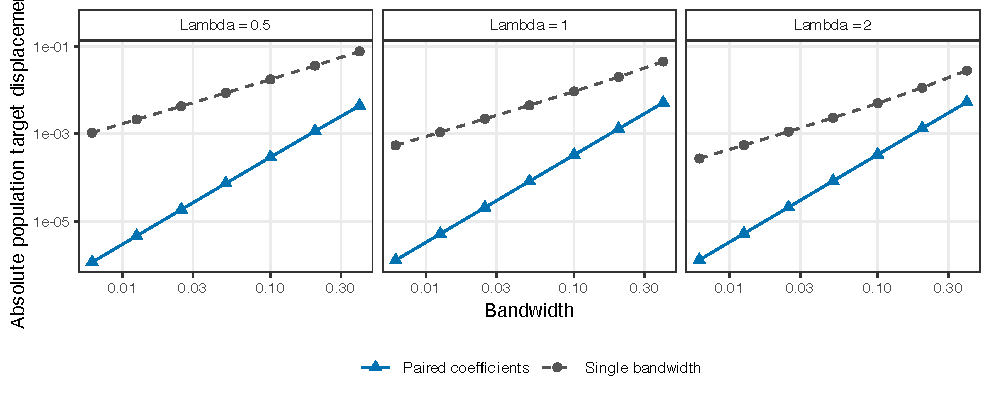
\includegraphics[width=\textwidth]{generated/figures/fig_joint_smoothing.pdf}
\caption{Population coefficient displacement in the repeated observation
model at the lower quartile. Both axes use logarithmic scales. Circles
show a single bandwidth and triangles show the paired coefficient
$2\beta_{h/2}-\beta_h$. Each panel fixes the nuisance penalty. The
points are deterministic integral calculations; an independent
Gauss--Legendre quadrature checks the population score.
The R plotting code was developed with OpenAI Codex.}
\label{fig:joint-smoothing}
\end{figure}

\subsection{Registered study of full target inference}\label{subsec:registered-study}

The registered statistical study contains \RegisteredJointSettings{}
settings and \RegisteredJointDatasets{} generated datasets.
Independent clusters follow
\[
 Y_{ij}=X_{ij}^T\beta^0+Z_{ij}^Tb_i+\varepsilon_{ij},
\]
with additional specified terms in the nuisance-misspecification
settings. The default design has Gaussian AR(1) covariates with
correlation $0.5$, cluster sizes from three through eight, and
alternating nonzero coefficients of magnitude $0.75$. The
configurations vary sample size and dimension before examining
innovation distributions and cluster heterogeneity. Their covariance
and signal settings test the adjustment step, while a separate
group varies the working penalty and learning budget. Most settings
use all generated predictors. Five prescreening settings examine
how the available predictor set affects the inferential target.
Supporting Information specifies every generating distribution and
the 500 or 1000 replications assigned to each setting.

The full profile target is calculated independently whenever its
equality with the generating slope is unavailable. Four population
repetitions, each containing at least 100000 clusters, determine
these targets and their Monte Carlo errors. The sample algorithm
uses its fixed training rules and never receives those population
calculations. Two active and two null coordinates are requested
in every statistical dataset.

Table~\ref{tab:registered-joint-overview} reports coverage of the
full target. Each setting contributes equally within its declared
input category, and the parentheses give Monte Carlo standard errors
based on replication averages. The fits column records numerical
completion. The \RegisteredJointFailures{} unavailable fits remain
in the coverage denominator. The complete setting-level results and
interval lengths appear in Supporting Information.

\begin{table}

\caption{\label{tab:registered-joint-overview}Full target coverage by the declared predictor input}
\centering
\begin{tabular}[t]{lrlll}
\toprule
Input & Settings & Fits & Active & Null\\
\midrule
Full predictor set & 66 & 42994/43000 & 0.971 (0.001) & 0.977 (0.001)\\
Independent screening & 3 & 1500/1500 & 0.958 (0.004) & 0.975 (0.003)\\
Same sample screening & 1 & 500/500 & 0.981 (0.004) & 0.979 (0.005)\\
Variance filtering & 1 & 500/500 & 0.661 (0.012) & 0.694 (0.012)\\
\bottomrule
\end{tabular}
\end{table}


Variance filtering changes the target in a reproducible way. In
F05, it retains 300 of the 5000 predictors by their observed variance
and adds the requested coordinates. Active and null coverage are
\VarianceFilterActiveCoverage{} and \VarianceFilterNullCoverage{}.
The exact Gaussian projection of each saved selected model shows
a displacement of the second coordinate in
\VarianceFilterSecondShifted{} of 500 datasets and of the eleventh
coordinate in \VarianceFilterEleventhShifted{} datasets. Both
coordinates have conditional adjustments outside the retained pool.
The full-design setting F06 has coverages
\FullDesignActiveCoverage{} and \FullDesignNullCoverage{}, and
every requested selected target agrees with its full-design value
within $10^{-8}$. These calculations locate the coverage loss in
the parameter change induced by prescreening.

\subsection{Independent assessment of conditional adjustment}\label{subsec:sim-design}

An independent ablation study contains 24 settings, each with
60 independent datasets from the same model form.
Cluster sizes are sampled uniformly from three through eight.
Covariate rows are centred Gaussian with
$\Sigma_{kl}=\rho_X^{|k-l|}$, independent of the cluster effects and
innovations. Five nonzero coefficients alternate in sign. Their
reference magnitude is $0.75$, with $0.40$ in the weak-signal settings.
The random-intercept standard deviation is one. For $q=2$, the
random-slope standard deviation is $0.5$ and the two effects have
correlation $0.4$.

The reference settings cross $n\in\{200,400\}$,
$q\in\{1,2\}$ and $\tau\in\{0.25,0.50,0.75\}$ at $p=500$.
Additional settings use standardised $t_3$ innovations, smaller
signals, covariate correlation $0.8$, and $p=1000$ or $2000$.
Every innovation is centred at its specified quantile. The complete
configuration table appears in Supporting Information. Centred
Gaussian designs satisfy the profile orthogonality identity, so the
full population slope target equals $\beta^0$ in these settings.
Coordinates 1 and 2 assess nonzero coefficients; coordinates 6 and 7
assess zero coefficients.

All tuning uses training data and the rules in
Section~\ref{sec:inference}, with $\Lambda=I$ and $h=n^{-3/10}$.
The procedure was fixed before this independent evaluation. The
resulting \JointDatasets{} datasets provide \JointIntervals{}
requested intervals, all of which were computed. Each replication
contributes its mean coverage within the active or null coordinate
group. Monte Carlo standard errors use these replication averages
and retain the scenario strata. Coordinatewise exact binomial
intervals are reported separately in Supporting Information.

\label{subsec:sim-comparators}

A paired ablation removes $S_{fk}^X$ from
\eqref{eq:selected-set}. It retains the outcome search, profile
adjustment, bandwidths, coefficient fits and variance formula. Both
procedures use the same generated datasets and subject partitions.
This comparison tests whether conditional covariates recover
adjustments that the outcome and profile searches omit.

Table~\ref{tab:joint-simulation} reports coverage together with interval
length. Across all settings, active-coordinate coverage is
\JointActiveCoverage{} with Monte Carlo standard error
\JointActiveMCSE{}. Null-coordinate coverage is
\JointNullCoverage{} with standard error \JointNullMCSE{}.
The corresponding ablation coverages are
\JointActiveAblationCoverage{} and \JointNullAblationCoverage{}.
For active coordinates, the paired coverage difference is
\JointActiveCoverageDifference{} with Monte Carlo standard error
\JointActiveDifferenceMCSE{}.

The effect is concentrated in the smaller-signal settings. Their
active-coordinate coverage is \JointWeakCoverage{} for the complete
procedure and \JointWeakAblationCoverage{} for the ablation, a paired
difference of \JointWeakDifference{} with standard error
\JointWeakDifferenceMCSE{}. The exact Gaussian projection formula
also identifies \JointAblationShiftCount{} ablated coordinate fits
whose fold-averaged population target differs from the full target by
more than $10^{-8}$. The largest absolute shift is
\JointAblationMaxShift{}. Every selected coordinate target of the
complete procedure agrees with the full target at that tolerance.

\begin{table}[t]
\caption{Coverage and interval length with paired removal of design adjustment}\label{tab:joint-simulation}
\centering\small
\begin{tabular}{lrrrrr}
\toprule
Setting & Coordinate & Full coverage & Ablation & Difference & Length \\
\midrule
$t_3$ errors & Active & 0.963 (0.009) & 0.948 (0.010) & 0.015 (0.008) & 0.249 / 0.232 \\
$t_3$ errors & Null & 0.963 (0.008) & 0.960 (0.009) & 0.002 (0.009) & 0.290 / 0.257 \\
Correlation 0.8 & Active & 0.975 (0.014) & 0.983 (0.012) & -0.008 (0.015) & 0.489 / 0.472 \\
Correlation 0.8 & Null & 0.967 (0.016) & 0.975 (0.014) & -0.008 (0.015) & 0.568 / 0.545 \\
Gaussian n200 & Active & 0.968 (0.007) & 0.956 (0.008) & 0.013 (0.007) & 0.312 / 0.299 \\
Gaussian n200 & Null & 0.969 (0.007) & 0.964 (0.007) & 0.006 (0.007) & 0.367 / 0.327 \\
Gaussian n400 & Active & 0.964 (0.007) & 0.950 (0.009) & 0.014 (0.006) & 0.203 / 0.190 \\
Gaussian n400 & Null & 0.971 (0.006) & 0.961 (0.007) & 0.010 (0.007) & 0.222 / 0.209 \\
Larger dimension & Active & 0.958 (0.009) & 0.958 (0.010) & 0.000 (0.009) & 0.253 / 0.238 \\
Larger dimension & Null & 0.965 (0.009) & 0.950 (0.011) & 0.015 (0.008) & 0.287 / 0.261 \\
Weak signals & Active & 0.958 (0.010) & 0.803 (0.022) & 0.156 (0.022) & 0.338 / 0.308 \\
Weak signals & Null & 0.972 (0.009) & 0.922 (0.014) & 0.050 (0.014) & 0.386 / 0.341 \\
\bottomrule
\end{tabular}
\par\smallskip\parbox{\textwidth}{\footnotesize Parentheses give Monte Carlo standard errors. Differences use the same generated datasets. Length lists the full procedure followed by the ablation. Each dataset contributes two active and two null coordinates; standard errors use averages within datasets and retain the scenario strata.}
\end{table}


The adjustment has a precision cost. Mean active-coordinate interval
length increases from \JointActiveAblationLength{} to
\JointActiveLength{}, and the corresponding null-coordinate lengths
are \JointNullAblationLength{} and \JointNullLength{}. The complete
procedure therefore spends precision to retain the desired coordinate
when selection omits part of the outcome model. The correlation and
larger-dimension settings in Table~\ref{tab:joint-simulation} also
show that the coverage difference varies across configurations.

\subsection{Growing sample size and influence approximation}\label{subsec:sim-influence}
\newcommand{\GaussianDiagnosticDatasets}{10500}
\newcommand{\GaussianRemainderFiveSmall}{0.774}
\newcommand{\GaussianRemainderFiveLarge}{0.347}
\newcommand{\GaussianRemainderTenSmall}{1.159}
\newcommand{\GaussianRemainderTenLarge}{0.387}
\newcommand{\GaussianCurvatureIntegral}{0.3117484}
\newcommand{\GaussianCurvaturePopulation}{0.3119884}
\newcommand{\GaussianCurvatureMCSE}{0.0005868}
\newcommand{\GaussianCurvatureClusters}{100000}


The registered scaling settings vary $n\in\{100,200,400\}$ and
$p\in\{500,1000,2000\}$ with five active coefficients. An additional
sequence has ten active coefficients at $p=1000$. These twelve
settings use Gaussian innovations, a random intercept, covariate
correlation $0.5$ and the median quantile. Each setting has 1000
independent replications, except those at $p=2000$, which have 500.
All \GaussianDiagnosticDatasets{} datasets complete the proposed fit.

The Gaussian design permits a direct evaluation of the population
inverse row through the Stein calculation in Supporting Information.
We use it to evaluate the cluster contribution in
\eqref{eq:influence} at the generating coefficient. The scaled
remainder subtracts its sample average from the coefficient error
and multiplies the difference by $\sqrt n$.
Figure~\ref{fig:gaussian-influence} shows the root mean squared
remainder together with Hessian and inverse-row errors. At $p=1000$
and $s=5$, the remainder decreases from
\GaussianRemainderFiveSmall{} at 100 clusters to
\GaussianRemainderFiveLarge{} at 400. The corresponding values
with ten active coefficients are \GaussianRemainderTenSmall{}
and \GaussianRemainderTenLarge{}. The selected Gaussian targets
agree with the requested full-design coordinates within $10^{-8}$
in every estimation fold. The remaining approximation error thus
comes from estimation of the selected coefficients and their
influence representation in these settings.

\begin{figure}[t]
\centering
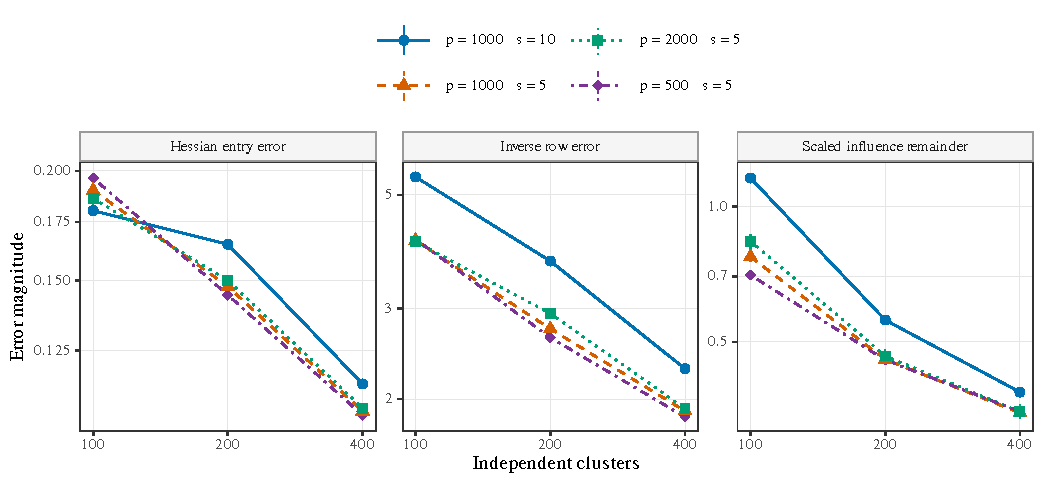
\includegraphics[width=\textwidth]{generated/figures/fig_gaussian_influence_diagnostics.pdf}
\caption{Gaussian scaling diagnostics for the proposed estimator.
The left panel gives the mean maximum-entry error of the selected
Hessian evaluated at the full target. The middle panel gives the
mean Euclidean error of each fitted inverse row relative to its
unsmoothed population row. Both averages include the two bandwidths,
estimation folds and requested coordinates. The right panel gives
the root mean squared scaled influence remainder. Colours and
symbols identify the dimension and sparsity settings. Bars show
1.96 Monte Carlo standard errors on either side of each estimate;
both axes use logarithmic scales. The R plotting code was developed
with OpenAI Codex.}
\label{fig:gaussian-influence}
\end{figure}

\subsection{Computational scaling}\label{subsec:sim-metrics}

Twenty timed repetitions at each dimension use $n=200$, $q=1$,
$\tau=0.50$ and four requested coordinates. Table~\ref{tab:joint-runtime}
reports single-process elapsed fitting time on an ARM64 macOS
computer with R 4.3.2, excluding data generation. The median
is \JointRuntimeFiveHundred{} seconds at $p=500$ and
\JointRuntimeTenThousand{} seconds at $p=10000$. Most computation
occurs in the selection samples; the final two-bandwidth fits involve
only their selected coordinate sets. These measurements include
profile and conditional covariate selection, so they measure the
implemented statistical procedure.

\begin{table}[t]
\caption{Seconds for four requested coordinates at two hundred clusters}\label{tab:joint-runtime}
\centering\small
\begin{tabular}{lrrrrr}
\toprule
$p$ & Repetitions & Median & 90th percentile & Maximum & Inference \\
\midrule
  500 & 20 & 0.966 & 1.006 & 1.253 & 0.023 \\
 1000 & 20 & 1.734 & 1.839 & 1.864 & 0.027 \\
 2000 & 20 & 2.820 & 3.095 & 3.256 & 0.029 \\
10000 & 20 & 9.976 & 10.606 & 10.676 & 0.031 \\
\bottomrule
\end{tabular}
\end{table}


\newcommand{\SubmissionTimingReplications}{350}
\newcommand{\SubmissionTimingJointHigh}{3.031}
\newcommand{\SubmissionTimingPooledHigh}{80.340}
\newcommand{\SubmissionTimingTwelve}{4.471}
\newcommand{\SubmissionWallFour}{331.943}
\newcommand{\SubmissionWallEight}{197.697}

The registered computation study adds fifty repetitions in each of
seven settings, including random slopes, prescreening and twelve
requested coordinates. At $n=200$ and $p=2000$, median time for the
complete four-coordinate procedure is
\SubmissionTimingJointHigh{} seconds. Pooled quantile Lasso takes
\SubmissionTimingPooledHigh{} seconds for its tuning and fit on
the same datasets. The twelve-coordinate procedure at $n=200$ and
$p=1000$ takes \SubmissionTimingTwelve{} seconds. Supporting
Information reports the complete timing distributions and the
four-worker and eight-worker calculations with identical data
and tuning seeds.

\section{Milk spectra and somatic cell score}\label{sec:application}

\subsection{Repeated measurements and the coordinate of interest}

The public milk dataset \cite{chirife2025data} combines mid-infrared (MIR)
spectra, milk protein genotypes and somatic cell counts from six
commercial Holstein-Friesian farms in Catalonia. Each spectrum
contains \MilkSpectra{} recorded absorbance variables. A MilkoScan
7RM measured the spectrum, and a separate Fossomatic instrument
measured somatic cell count. The cow identifier links observations
across two routine milk controls.

We study the association of A2 milk type with somatic cell score
after adjustment for the complete recorded spectrum and the sampling
conditions. Associations between milk protein genotypes and somatic
cell score have previously been examined with repeated-measurement
mixed models \cite{citek2022}. Here the coefficient is a coordinate
of the full high-dimensional profile target at each quantile.
The indicator $A2_i$ equals one for genotype A2A2 and zero for
A1A1 or A1A2. With count recorded in cells per microlitre, the
response is
\[
 Y_{ij}=\log_2(\mathrm{SCC}_{ij}/100)+3.
\]
This transformation retains the recorded measurement precision.

Requiring consistent cow identifiers, genotypes and sampling occasions
retains \MilkCows{} cows and \MilkSamples{} milk samples. Of these,
\MilkRepeatCows{} cows contribute two observations; the remaining cows
contribute one. Counts and all spectral measurements are observed for
every retained record. There are \MilkATwoCows{} A2 cows and
\MilkAOneCows{} A1 cows, with both milk types represented at every farm.
The profile criterion gives each cow the same total weight.

The cow-weighted marginal SCS medians are $\MilkAOneMedian{}$ for A1
and $\MilkATwoMedian{}$ for A2. These summaries average over the
recorded milk spectra and sampling conditions. Supporting Information
reports the full descriptive distributions before the conditional
profile analysis.

\subsection{Full spectrum adjustment and inference}

The fixed design contains $A2_i$, twelve indicators for the observed
farm and milk-control combinations, and all \MilkSpectra{} spectral
variables. Its dimension is \MilkDimension{}. The milk-type indicator
and sampling-condition indicators are always included. We use a cow
intercept, $Z_{ij}=1$, with fixed $\Lambda=1$ and
$h=n^{-3/10}$ at $\tau=0.25,0.50,0.75$.

A fixed random ordering assigns complete cows to two groups. For each
estimation group, the complementary cows supply the outcome search,
profile-curvature adjustment and conditional covariate adjustment of
Section~\ref{sec:inference}. The resulting selected model is fitted
at $h$ and $h/2$. The two groups contain 674 and 675 cows, so the full
design dimension exceeds the number of cows in either estimation
group. All spectral variables remain available to the selection
procedure. The interval addresses the complete-spectrum population
coordinate under the target-approximation conditions of
Section~\ref{sec:theory}.

Adjacent spectral measurements are strongly related: their median
correlation is \MilkSpectralCorrelation{}. Gaussian Lasso subproblems
use covariance updates and retain the declared validation grids.
The selected convex fits use a cluster-weighted QR representation,
with the coefficient and inverse direction transformed back to the
recorded covariate units. This invertible transformation preserves
the profile objective and its prediction ridge. All fitted gradients
are checked in the original coordinates.

\subsection{Estimated milk type associations}

\begin{table}[t]
\centering
\caption{A2 milk profile coefficients for somatic cell score with all 1060 MIR variables available for adjustment. The pointwise intervals have 95\% confidence level. Simultaneous intervals allocate 5\% across the three fixed quantiles. All fits use a cow intercept and $\Lambda=1$.}
\label{tab:milk-inference}
\begin{tabular}{rrrrr}
\toprule
$\tau$ & Estimate & Standard error & Pointwise interval & Simultaneous interval \\
\midrule
0.25 & -0.020 & 0.101 & $[-0.219,\ 0.179]$ & $[-0.263,\ 0.223]$ \\
0.50 & 0.018 & 0.118 & $[-0.213,\ 0.248]$ & $[-0.264,\ 0.299]$ \\
0.75 & 0.119 & 0.140 & $[-0.155,\ 0.393]$ & $[-0.216,\ 0.453]$ \\
\bottomrule
\end{tabular}
\end{table}


After adjustment for the measured spectrum and sampling conditions,
no A2 coefficient is statistically distinguishable from zero at the
simultaneous confidence level. The median
coefficient is $\MilkMedianEstimate{}$, with simultaneous
interval $\MilkMedianInterval{}$. The lower-quartile estimate is
$\MilkLowerEstimate{}$ and the upper-quartile estimate is
$\MilkUpperEstimate{}$. All three simultaneous intervals include zero.
Table~\ref{tab:milk-inference} reports their standard errors and both
interval families. The simultaneous intervals allocate 5\% across
the three prespecified quantiles and use the joint cluster
contributions of both bandwidths. The median interval, for example,
allows changes of approximately three tenths of an SCS unit in either
direction.

The supplementary comparison of quantiles uses their common cow
influence values. The upper-minus-lower coefficient difference is
$\MilkUpperLowerDifference{}$, with simultaneous interval
$\MilkUpperLowerDifferenceInterval{}$. A joint Wald test of equality
of the three coefficients gives $p=\MilkQuantileEqualityP{}$.
Variation of the adjusted milk-type association across these three
quantiles is also unresolved by this sample.

\subsection{Sensitivity and numerical behaviour}

Bandwidth multipliers $0.75$ and $1.25$ produce a largest absolute
change of $\MilkMaxBandwidthChange{}$ SCS units in the reference
coefficients. All their simultaneous intervals include zero. The
working-penalty settings $\Lambda=0.5$ and $2$ likewise yield intervals
containing zero for their respective profile targets. Supporting
Information reports every estimate and interval.

Restricting the analysis to cows with two milk controls changes the
median estimate to $\MilkPairedMedianEstimate{}$, with interval
$\MilkPairedMedianInterval{}$. The restriction also changes the
observed outcome distribution: cows with one control have mean SCS
$\MilkSingleMean{}$, compared with $\MilkRepeatedMean{}$ among cows
with two controls under equal cow weighting.

All \MilkFits{} registered fits and their \MilkSystems{} constituent
coefficient systems are available. Selected dimensions range from
\MilkMinSelected{} to \MilkMaxSelected{} across the estimation
groups. Median coordinate-fitting time is \MilkMedianRuntime{}
seconds after the common design regressions have been computed.
The numerical records retain original-coordinate gradients and
nuisance gradients, together with the selected sets and the influence
values used to reconstruct every standard error.

Inference treats cows as independent conditional on the farm and
milk-control indicators. The six farms define the observed sampling
conditions. The public file does not record days in milk, parity or
pedigree, so these variables are outside the observed adjustment set.
The complete workflow and its numerical checks are available with
the replication files.

\section{Discussion}\label{sec:discussion}

A computationally useful high-dimensional profile estimator must
retain the meaning of the requested coordinate after reducing the
design. The selected-target bound makes that requirement explicit:
outcome approximation enters quadratically, and its interaction with
the adjustment contrast contributes a product term. Conditional
covariate selection has a direct interpretation in Gaussian designs,
where retaining a coordinate's conditional neighbours preserves its
population slope even when other outcome coefficients are omitted.
The paired ablation illustrates the consequence for smaller signals,
where predictive selection alone gives limited incentive to retain
those adjustments.

Bounded cluster sizes create a separate smoothing effect. The cluster
nuisance optimiser moves with the bandwidth, producing a linear term
in the population profile expansion. Pairing two fitted coefficient
vectors removes this term. Positive curvature is retained in both
constituent fits, and their cluster contributions determine the
covariance of the combined estimator. This construction supports
practical calculation while preserving a complete profile target
defined independently of the numerical bandwidth.

The milk analysis estimates a fixed milk-type coordinate with the
complete spectrum available for adjustment. Its three simultaneous
intervals include zero, while retaining uncertainty about associations
of either sign. Strong correlations between adjacent spectral variables
make stable computation consequential: the weighted QR calculation
preserves the declared profile and returns the coefficient to its
original units. Interpretation conditions on the measured spectrum
and the observed farm and milk-control combinations.

The theory uses independent clusters, bounded cluster sizes and a
fixed positive-definite nuisance matrix. Learning that matrix for an
inferential parameter would add its estimation contribution to the
population expansion and influence representation. The current
selected-model argument permits imperfect outcome selection and
growing dimension through explicit approximation rates. Extending
the coordinate process to an increasing number of targets would
require a uniform Gaussian approximation and a matching simultaneous
variance construction.

\section*{Acknowledgements}
The authors thank colleagues and seminar participants for comments on earlier versions of the project.
OpenAI Codex assisted with manuscript drafting and language editing.


\section*{Conflict of interest}
The authors declare no conflict of interest.


\section*{Data availability statement}
The soybean data are publicly distributed in the R packages
\texttt{NAM} version 1.8.0 and \texttt{SoyNAM} version 1.6.2.
The analysis uses the \texttt{met} and \texttt{soyin} data objects;
their source revisions and variable reconciliation are recorded with
the replication materials. The measurement design is described by
\citeA{xavier2017canopy}. Analysis code and aggregate results are
available at \url{https://github.com/Stork343/jpDMEQR/tree/recovery/research-20261028}.
The replication scripts retrieve the pinned source objects and generate
the complete analysis panel, numerical checks and manuscript tables.


\section*{Supporting information}
The accompanying supplement contains the profile calculus and proofs, followed by the computational specification and extended numerical results. Its milk spectra section gives the cohort construction, sample roles, equivalent numerical coordinates and all sensitivity intervals.

\bibliography{references}

\bigskip
\noindent Jian Hou, School of Statistics, Renmin University of China, Beijing, China.
Email: \texttt{houjian@ruc.edu.cn}.

\end{document}

